\documentclass[]{article}
\usepackage{lmodern}
\usepackage{amssymb,amsmath}
\usepackage{ifxetex,ifluatex}
\usepackage{fixltx2e} % provides \textsubscript
\ifnum 0\ifxetex 1\fi\ifluatex 1\fi=0 % if pdftex
  \usepackage[T1]{fontenc}
  \usepackage[utf8]{inputenc}
\else % if luatex or xelatex
  \ifxetex
    \usepackage{mathspec}
  \else
    \usepackage{fontspec}
  \fi
  \defaultfontfeatures{Ligatures=TeX,Scale=MatchLowercase}
\fi
% use upquote if available, for straight quotes in verbatim environments
\IfFileExists{upquote.sty}{\usepackage{upquote}}{}
% use microtype if available
\IfFileExists{microtype.sty}{%
\usepackage{microtype}
\UseMicrotypeSet[protrusion]{basicmath} % disable protrusion for tt fonts
}{}
\usepackage[margin=1in]{geometry}
\usepackage{hyperref}
\hypersetup{unicode=true,
            pdftitle={Food Intake Analysis of NCD/HFD Dexamethasone Treated Animals},
            pdfauthor={Dave Bridges and Innocence Harvey},
            pdfborder={0 0 0},
            breaklinks=true}
\urlstyle{same}  % don't use monospace font for urls
\usepackage{color}
\usepackage{fancyvrb}
\newcommand{\VerbBar}{|}
\newcommand{\VERB}{\Verb[commandchars=\\\{\}]}
\DefineVerbatimEnvironment{Highlighting}{Verbatim}{commandchars=\\\{\}}
% Add ',fontsize=\small' for more characters per line
\usepackage{framed}
\definecolor{shadecolor}{RGB}{248,248,248}
\newenvironment{Shaded}{\begin{snugshade}}{\end{snugshade}}
\newcommand{\KeywordTok}[1]{\textcolor[rgb]{0.13,0.29,0.53}{\textbf{{#1}}}}
\newcommand{\DataTypeTok}[1]{\textcolor[rgb]{0.13,0.29,0.53}{{#1}}}
\newcommand{\DecValTok}[1]{\textcolor[rgb]{0.00,0.00,0.81}{{#1}}}
\newcommand{\BaseNTok}[1]{\textcolor[rgb]{0.00,0.00,0.81}{{#1}}}
\newcommand{\FloatTok}[1]{\textcolor[rgb]{0.00,0.00,0.81}{{#1}}}
\newcommand{\ConstantTok}[1]{\textcolor[rgb]{0.00,0.00,0.00}{{#1}}}
\newcommand{\CharTok}[1]{\textcolor[rgb]{0.31,0.60,0.02}{{#1}}}
\newcommand{\SpecialCharTok}[1]{\textcolor[rgb]{0.00,0.00,0.00}{{#1}}}
\newcommand{\StringTok}[1]{\textcolor[rgb]{0.31,0.60,0.02}{{#1}}}
\newcommand{\VerbatimStringTok}[1]{\textcolor[rgb]{0.31,0.60,0.02}{{#1}}}
\newcommand{\SpecialStringTok}[1]{\textcolor[rgb]{0.31,0.60,0.02}{{#1}}}
\newcommand{\ImportTok}[1]{{#1}}
\newcommand{\CommentTok}[1]{\textcolor[rgb]{0.56,0.35,0.01}{\textit{{#1}}}}
\newcommand{\DocumentationTok}[1]{\textcolor[rgb]{0.56,0.35,0.01}{\textbf{\textit{{#1}}}}}
\newcommand{\AnnotationTok}[1]{\textcolor[rgb]{0.56,0.35,0.01}{\textbf{\textit{{#1}}}}}
\newcommand{\CommentVarTok}[1]{\textcolor[rgb]{0.56,0.35,0.01}{\textbf{\textit{{#1}}}}}
\newcommand{\OtherTok}[1]{\textcolor[rgb]{0.56,0.35,0.01}{{#1}}}
\newcommand{\FunctionTok}[1]{\textcolor[rgb]{0.00,0.00,0.00}{{#1}}}
\newcommand{\VariableTok}[1]{\textcolor[rgb]{0.00,0.00,0.00}{{#1}}}
\newcommand{\ControlFlowTok}[1]{\textcolor[rgb]{0.13,0.29,0.53}{\textbf{{#1}}}}
\newcommand{\OperatorTok}[1]{\textcolor[rgb]{0.81,0.36,0.00}{\textbf{{#1}}}}
\newcommand{\BuiltInTok}[1]{{#1}}
\newcommand{\ExtensionTok}[1]{{#1}}
\newcommand{\PreprocessorTok}[1]{\textcolor[rgb]{0.56,0.35,0.01}{\textit{{#1}}}}
\newcommand{\AttributeTok}[1]{\textcolor[rgb]{0.77,0.63,0.00}{{#1}}}
\newcommand{\RegionMarkerTok}[1]{{#1}}
\newcommand{\InformationTok}[1]{\textcolor[rgb]{0.56,0.35,0.01}{\textbf{\textit{{#1}}}}}
\newcommand{\WarningTok}[1]{\textcolor[rgb]{0.56,0.35,0.01}{\textbf{\textit{{#1}}}}}
\newcommand{\AlertTok}[1]{\textcolor[rgb]{0.94,0.16,0.16}{{#1}}}
\newcommand{\ErrorTok}[1]{\textcolor[rgb]{0.64,0.00,0.00}{\textbf{{#1}}}}
\newcommand{\NormalTok}[1]{{#1}}
\usepackage{longtable,booktabs}
\usepackage{graphicx,grffile}
\makeatletter
\def\maxwidth{\ifdim\Gin@nat@width>\linewidth\linewidth\else\Gin@nat@width\fi}
\def\maxheight{\ifdim\Gin@nat@height>\textheight\textheight\else\Gin@nat@height\fi}
\makeatother
% Scale images if necessary, so that they will not overflow the page
% margins by default, and it is still possible to overwrite the defaults
% using explicit options in \includegraphics[width, height, ...]{}
\setkeys{Gin}{width=\maxwidth,height=\maxheight,keepaspectratio}
\IfFileExists{parskip.sty}{%
\usepackage{parskip}
}{% else
\setlength{\parindent}{0pt}
\setlength{\parskip}{6pt plus 2pt minus 1pt}
}
\setlength{\emergencystretch}{3em}  % prevent overfull lines
\providecommand{\tightlist}{%
  \setlength{\itemsep}{0pt}\setlength{\parskip}{0pt}}
\setcounter{secnumdepth}{0}
% Redefines (sub)paragraphs to behave more like sections
\ifx\paragraph\undefined\else
\let\oldparagraph\paragraph
\renewcommand{\paragraph}[1]{\oldparagraph{#1}\mbox{}}
\fi
\ifx\subparagraph\undefined\else
\let\oldsubparagraph\subparagraph
\renewcommand{\subparagraph}[1]{\oldsubparagraph{#1}\mbox{}}
\fi

%%% Use protect on footnotes to avoid problems with footnotes in titles
\let\rmarkdownfootnote\footnote%
\def\footnote{\protect\rmarkdownfootnote}

%%% Change title format to be more compact
\usepackage{titling}

% Create subtitle command for use in maketitle
\newcommand{\subtitle}[1]{
  \posttitle{
    \begin{center}\large#1\end{center}
    }
}

\setlength{\droptitle}{-2em}
  \title{Food Intake Analysis of NCD/HFD Dexamethasone Treated Animals}
  \pretitle{\vspace{\droptitle}\centering\huge}
  \posttitle{\par}
  \author{Dave Bridges and Innocence Harvey}
  \preauthor{\centering\large\emph}
  \postauthor{\par}
  \predate{\centering\large\emph}
  \postdate{\par}
  \date{2017-08-08}


\begin{document}
\maketitle

{
\setcounter{tocdepth}{2}
\tableofcontents
}
\section{Purpose}\label{purpose}

To test whether food intake is different betwen NCD and HFD animals
treated with dexamethasone or water.

\section{Experimental Details}\label{experimental-details}

We monitored weekly food intake, at the cage level throughout the
experiment

\section{Raw Data}\label{raw-data}

Describe your raw data files, including what the columns mean (and what
units they are in).

These data can be found in
/Users/davebrid/Documents/GitHub/CushingAcromegalyStudy/scripts/scripts-obesity
in a file named ../../data/raw/HFD and NCD Food Intake Data.csv. This
script was most recently updated on Tue Aug 8 22:25:12 2017.

\section{Analysis}\label{analysis}

We converted NCD and HFD in grams to kcal by these factors

\begin{longtable}[]{@{}lr@{}}
\caption{Energy Density of Diets}\tabularnewline
\toprule
Diet & Calories per gram\tabularnewline
\midrule
\endfirsthead
\toprule
Diet & Calories per gram\tabularnewline
\midrule
\endhead
NCD & 2.91\tabularnewline
HFD & 4.73\tabularnewline
\bottomrule
\end{longtable}

\subsection{Weekly Data}\label{weekly-data}

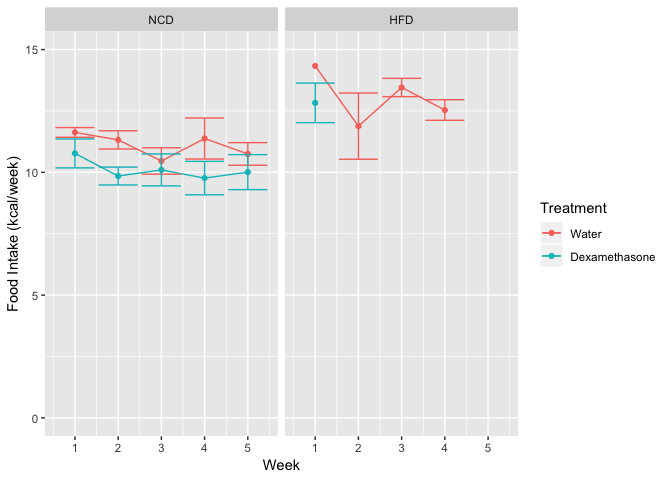
\includegraphics{figures/weekly-food-intake-1.png}

\subsection{Analysis on the Aggregate}\label{analysis-on-the-aggregate}

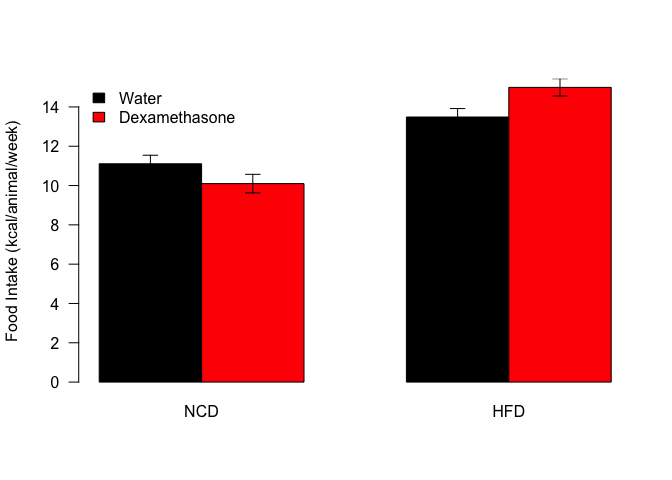
\includegraphics{figures/overall-food-intake-1.png}

\subsubsection{Aggregate Food Intake
Statistics}\label{aggregate-food-intake-statistics}

To analyse these data, we first aggregated the average food intake per
cage, assuming this did not change over time.

\begin{longtable}[]{@{}lrrrrr@{}}
\caption{Two-way ANOVA with Interaction for aggregated food
intake.}\tabularnewline
\toprule
term & df & sumsq & meansq & statistic & p.value\tabularnewline
\midrule
\endfirsthead
\toprule
term & df & sumsq & meansq & statistic & p.value\tabularnewline
\midrule
\endhead
Diet & 1 & 7.738 & 7.738 & 26.23 & 0.000\tabularnewline
Treatment & 1 & 0.354 & 0.354 & 1.20 & 0.276\tabularnewline
Diet:Treatment & 1 & 2.347 & 2.347 & 7.96 & 0.006\tabularnewline
Residuals & 96 & 28.324 & 0.295 & NA & NA\tabularnewline
\bottomrule
\end{longtable}

Based on this ANOVA there was a significant interaction between diet and
treatment, with HFD/Dexamethasone animals eating less food than
HFD/Water animals. We further analysed this via pairwiwse tests.

\begin{longtable}[]{@{}llr@{}}
\caption{Shapiro-Wilk test results for food intake
groups}\tabularnewline
\toprule
Diet & Treatment & Shapiro\tabularnewline
\midrule
\endfirsthead
\toprule
Diet & Treatment & Shapiro\tabularnewline
\midrule
\endhead
NCD & Water & 0.137\tabularnewline
NCD & Dexamethasone & 0.359\tabularnewline
HFD & Water & 0.563\tabularnewline
HFD & Dexamethasone & 0.438\tabularnewline
\bottomrule
\end{longtable}

Based on these tests, normality could be assumed for eachg group.

Based on Levene's tests, HFD (p=0.613) and NCD (p=0.71) could be assumed
to have equal variance.

We therefore performed Student's \emph{t}-tests with the following
results

\begin{longtable}[]{@{}lrrrrrrrll@{}}
\caption{Pairwise Student's t-test for the effects of dexamethasone on
food intake}\tabularnewline
\toprule
& estimate1 & estimate2 & statistic & p.value & parameter & conf.low &
conf.high & method & alternative\tabularnewline
\midrule
\endfirsthead
\toprule
& estimate1 & estimate2 & statistic & p.value & parameter & conf.low &
conf.high & method & alternative\tabularnewline
\midrule
\endhead
NCD & 11.1 & 10.1 & 2.97 & 0.006 & 28 & 0.314 & 1.704 & Two Sample
t-test & two.sided\tabularnewline
HFD & 13.5 & 15.0 & -2.19 & 0.032 & 68 & -2.928 & -0.138 & Two Sample
t-test & two.sided\tabularnewline
\bottomrule
\end{longtable}

The effects were significant in both cases, with HFD animals eating
slightly more food (11.181\% increase) and NCD animals eating slightly
less (-9.082\% decrease) food on a per calorie basis.

\section{Interpretation}\label{interpretation}

\section{Session Information}\label{session-information}

\begin{Shaded}
\begin{Highlighting}[]
\KeywordTok{sessionInfo}\NormalTok{()}
\end{Highlighting}
\end{Shaded}

\begin{verbatim}
## R version 3.3.0 (2016-05-03)
## Platform: x86_64-apple-darwin13.4.0 (64-bit)
## Running under: OS X 10.12.6 (unknown)
## 
## locale:
## [1] en_US.UTF-8/en_US.UTF-8/en_US.UTF-8/C/en_US.UTF-8/en_US.UTF-8
## 
## attached base packages:
## [1] stats     graphics  grDevices utils     datasets  methods   base     
## 
## other attached packages:
## [1] car_2.1-4     broom_0.4.2   ggplot2_2.2.1 forcats_0.2.0 readr_1.1.0  
## [6] dplyr_0.5.0   tidyr_0.6.1   knitr_1.15.1 
## 
## loaded via a namespace (and not attached):
##  [1] Rcpp_0.12.10       nloptr_1.0.4       highr_0.6         
##  [4] plyr_1.8.4         tools_3.3.0        digest_0.6.12     
##  [7] lme4_1.1-12        evaluate_0.10      tibble_1.3.0      
## [10] gtable_0.2.0       nlme_3.1-131       lattice_0.20-35   
## [13] mgcv_1.8-17        Matrix_1.2-8       psych_1.7.3.21    
## [16] DBI_0.6-1          yaml_2.1.14        parallel_3.3.0    
## [19] SparseM_1.76       stringr_1.2.0      MatrixModels_0.4-1
## [22] hms_0.3            rprojroot_1.2      grid_3.3.0        
## [25] nnet_7.3-12        R6_2.2.0           foreign_0.8-67    
## [28] rmarkdown_1.6      minqa_1.2.4        reshape2_1.4.2    
## [31] magrittr_1.5       splines_3.3.0      backports_1.0.5   
## [34] scales_0.4.1       htmltools_0.3.5    MASS_7.3-45       
## [37] assertthat_0.1     pbkrtest_0.4-7     mnormt_1.5-5      
## [40] colorspace_1.3-2   quantreg_5.29      labeling_0.3      
## [43] stringi_1.1.3      lazyeval_0.2.0     munsell_0.4.3
\end{verbatim}


\end{document}
